
\title{\LARGE\bf Low-latency localization by Active LED Markers tracking
\\
using a Dynamic Vision Sensor}


\author{Andrea Censi\mythanks, Jonas Strubel, Christian Brandli, Tobi Delbruck,
Davide Scaramuzza}
\maketitle
\begin{abstract}
At the current state of the art, the agility of an autonomous flying
robot is limited by its sensing pipeline, because the relatively high
latency and low sampling frequency limit the aggressiveness of the
control strategies that can be implemented. To obtain more agile robots,
we need faster sensing pipelines. A Dynamic Vision Sensor (DVS) is
a very different sensor than a normal CMOS camera: rather than providing
discrete frames like a CMOS camera, the sensor output is a sequence
of asynchronous timestamped events each describing a change in the
perceived brightness at a single pixel. The latency of such sensors
can be measured in the microseconds, thus offering the theoretical
possibility of creating a sensing pipeline whose latency is negligible
compared to the dynamics of the platform. However, to use these sensors
we must rethink the way we interpret visual data. This paper presents
a method for low-latency pose tracking using a DVS and Active Led
Markers (ALMs), which are LEDs blinking at high frequency (>1~KHz).
The sensor's time resolution allows distinguishing different frequencies,
thus avoiding the need for data association. This approach is compared
to traditional pose tracking based on a CMOS camera. The DVS performance
is not affected by fast motion, unlike the CMOS camera, which suffers
from motion blur. 
\end{abstract}

\section{Introduction}

Autonomous micro helicopters will soon play a major role in tasks
such search and rescue, environment monitoring, security surveillance,
inspection. A key problem in aerial-vehicle navigation is pose stabilization
and trajectory control in six degrees of freedom using onboard sensors.
Experiments with prototype systems that use an external motion-tracking
systems have shown that the platform themselves allow extreme maneuverability
if the localization problem can be assumed to be solved~\cite{Lupashin2012}.
However, such extreme performance is not attainable, not even in principle,
with traditional robotic sensors, such as CMOS cameras~\cite{Weiss2011}
or laser rangefinders~\cite{Shen2011}.

The agility of an autonomous flying robot is limited by the speed
of the sensing pipeline. More precisely, ``speed'' can be quantified
in observations\emph{ frequency} and \emph{latency} (\prettyref{fig:Discretization-and-latency}).
For a sensing pipeline based on a CMOS camera, the observations are
captured at a frequency on the order of 15--30~Hz and the total latency
of the pipeline, including both image acquisition and image processing
using common visual odometry approaches is in the order of 50--250~ms~\cite{Weiss2011}.
To obtain more agile systems, we need to use faster sensors and low-latency
processing.

This paper presents a method for pose tracking based on the use of
a Dynamic Vision Sensor (DVS). The main difference between a DVS and
a normal CMOS camera is that the DVS output is a stream of \emph{events}
that encode \emph{changes} in the brightness. Each event encodes
the location of the change, whether there was a positive or negative
change in brightness. The timestamp has a resolution in the order
of 1~$\mu$s.  These events are not unlike spikes in a biological
visual system; however, while retinal ganglion cells show latencies
of around 200~ms, the DVS chip has a latency of $15$~$\mu$s.

Theoretically, using a DVS we could obtain sensing pipelines with
a negligible latency compared to dynamics of the platform. We are
a few years to the goal, however. On the hardware side, the current
version of the DVS that is available commercially has a few limitations,
such as the limited resolution of $128\times128$ pixels, which is
the limiting factor for robotics applications.  It is projected
that in a couple of generations the technology will progress to have
comparable resolution with traditional cameras.

\begin{figure}[H]
\begin{centering}
\subfloat[Traditional architecture]{\begin{centering}
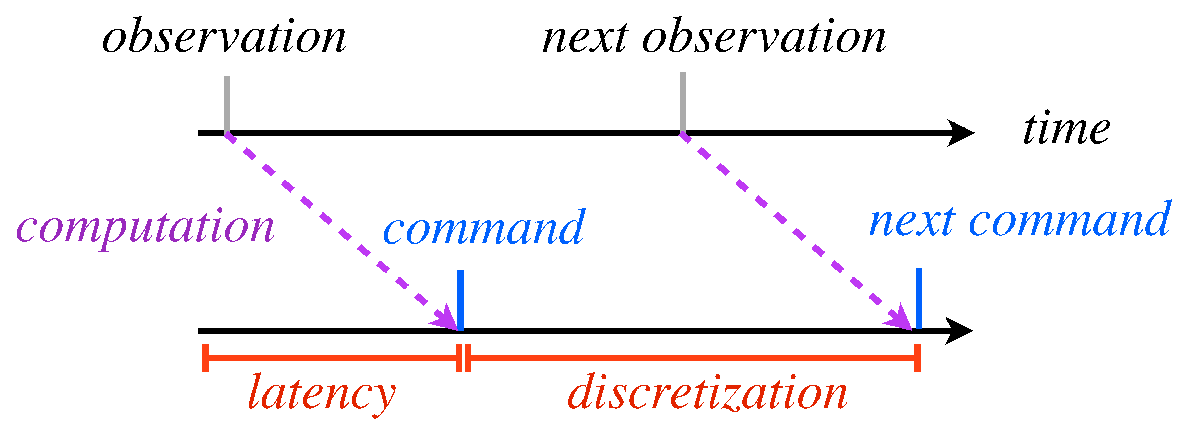
\includegraphics[width=8cm]{figures/slides/latency1}
\par\end{centering}

}
\par\end{centering}

\begin{centering}
\subfloat[Low latency, event-based architecture]{\begin{centering}
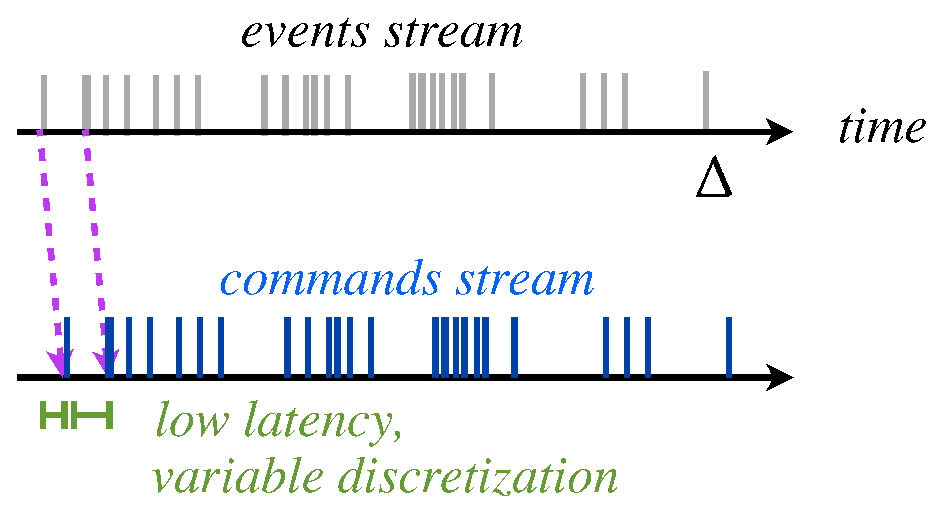
\includegraphics[width=8cm]{figures/slides/latency2}
\par\end{centering}

}
\par\end{centering}

\caption{\label{fig:Discretization-and-latency}To improve the agility of autonomous
flying robots, we need to improve the total latency of the sensing
pipeline. Using a device like a Dynamic Vision Sensor (DVS) we can
theoretically obtain a sensing pipeline which has microsecond latency.}
\end{figure}


On the theory side, to take full advantage of the sensor capability
we need to rethink completely the way we design robotic sensing pipelines.
In principle, it is possible to integrate the events of a DVS camera
to simulate a regular CMOS frame, and then adapt techniques from standard
image processing. However, that is not desirable, because it would
result in the same latency of a regular camera. Ideally, to have the
lowest latency for the sensing pipeline, one would want each single
event to be be reflected in a small but instantaneous change in the
commands given to the actuators. Therefore, our approach is to consider
methods that make use the information contained in each single event.

The pose-tracking method presented in this paper is based on using
Active LED Markers (\ALMs). These are infrared LEDs which are controlled
to blink at given known high frequencies, in the range of 1--2~$\,\mbox{kHz}$.
The DVS is fast enough to be able to distinguish different blinking
frequencies, so that, with proper processing, it is possible to also
uniquely assign an observable identity to each marker. We envision
that this system could be used for inter-robot localization for high-speed
acrobatic maneuvers, or that, in applications such as rescue robotics,
these markers could be left in the environment to facilitate cooperative
mapping.

One approach to using the DVS data is to cluster the events in order
to find spatio-temporal features, like points or lines, that are then
tracked through time~\cite{delbruck07fast,conradt09pencil,Matthias}.
This approach works well when the camera is static, because the output
is spatiotemporally sparse. The algorithm presented in this paper
uses a different approach. We found out that mounting a DVS camera
on a flying robot creates a new set of challenges. Because of the
apparent motion of the environment, the events are not spatiotemporally
sparse anymore. Moreover, while in controlled conditions the DVS camera
parameters can be tuned to obtain the best performance, a robot must
be able to work in a wider range of environmental conditions and be
robust to interferences. To achieve this robustness we have developed
an approach that sacrifices some latency to be more robust to noise
and unmodeled phenomena. We accumulate the events perceived in thin
slices of times corresponding to the blinking frequency ($1$~ms
slice for 1~kHz data). This allows to do detection of the \ALMs
position in image space. On top of this, we use a particle filter
for tracking the position in image space of each detection, and a
disambiguation stage to obtain coherent hypotheses on the joint position
of the markers. Finally, we reconstruct the pose using a standard
approach to rigid reconstruction.

Our method is evaluated in the application of tracking the pose of
a drone during an aggressive maneuver (a flip), and it is compared
to a more traditional approach, based on using a CMOS camera and a
feature-based visual odometry method. Experiments show that our method,
with a latency of $1$~ms, is able to reacquire tracking instantaneously
regardless of the fast motion, while the CMOS data is unusable for
visual odometry because it is corrupted by motion blur. We evaluate
the reconstruction accuracy using an OptiTrack system and find values
that are compatible with the low spatial resolution (128$\times$128)
of the DVS, which proves to be the current limitation of this approach.



Software, datasets, and videos illustrating the method are available
at the website \myurl.
